\section{Intrusion Detection Systems}
\emph{Intrusion detection systems} (IDS) are a brick in the existing defence algorithms arsenal wall of information security. More specifically, it comprises a series of mechanisms that monitor network nodes and detect intrusions, i.e. malicious activity or policy violations. An IDS usually analyses the incoming packets and notifies the suspect ones. In the most often cases, IDS are defined to be the sole surveillance application and does not comprise the control application: how the suspect packets are treated after a notification is not considered as being part of the IDS, the latter only focuses on the monitoring, analysis and notification \cite{Mukherjee1994NetworkDetection}. Classically, the reports are made to an administrator or another competent entity, as \emph{security information and event management} (SIEM) \cite{Bhatt2014TheSystems}, which are then in charge of the control application. 

IDS should not be confused with \emph{firewalls}, but merely be seen as a complement of it. The sole role of firewalls is to ensure that communication policies are followed carefully. A first
difference is that firewalls have an upstream role whereas IDS are working downstream. In other words, firewalls are verifying that each packet is following carefully one of the pre-defined allowed communication protocols, before it enters the local network. An IDS analyses the packets after they entered the local network to control if they shows no abnormal behaviour. Another second difference has already been mentioned: firewalls consider each packet separately whereas IDS can consider group of packets and thus look at a communication as whole. In this sense, IDS are much more suited against \emph{denial of service} (DoS) attacks than classical firewalls. A last difference concerns the exact scope of the packet analysis. As firewalls only have to enforce communication policies, they only have to look at the packet header, whereas IDS are searching for abnormal behaviours and are thus looking at the packets on their whole. To summarise this all, let's consider a high security building: the firewall would be equivalent to the agents allowing or not each individual to enter the site by carefully inspecting their papers, whereas the IDS would be the security agents monitoring the cameras inside to building searching for abnormal behaviour.

IDS should also not be confused with \emph{anti-viruses} application --- though the term \emph{anti-malware} would be more suited nowadays --- that refer to the application layer in charge of the detection and control of malicious code, or malware. The first difference concerns the scope of their analysis: anti-viruses are analysing (executable) code on a system more specifically than packets on a network. The second difference is similar as before: anti-viruses analyses code before it is allowed to be executed by the system and IDS are analysing packets that already entered the network.

However, all these taxonomy classifications are to be considered with some flexibility. As the attacks become more and more sophisticated, security entities are incorporating more and more subtleties are extending the scope of their detection methods. As such, they integrate other type of methods classically defined by other entities.

\subsection{How IDS work}
As briefly stated before, IDS have three main components: monitoring, analysis and notification. 

The monitoring can be achieved in real time or at regular interval on different types of nodes, which define the type of IDS: network based IDS (NIDS), host based IDS (HIDS) and hybrid of they monitor on both. 

The analysis is the core part of the IDS and is again divided in three main components: the extraction of features, the pattern analysis and the final classification \cite{Winter2018}. This will be the part which will interest us in this thesis.

As written before, the notification is done to a controller, either ban administrator or a SIEM. Classically, this takes place as the form of a series of logs which are later examined by the controller. In this sense, the speed is not the main focus of an IDS, but rather the correct identification of intrusions. However, one can also consider \emph{intrusion prevention systems} (IPS) which are working upstream. The literature sometimes consider these systems to be a specific class of IDS or to be a category on their own. However in opposition to IDS, IPS need to be fast and thus usually use signature-based detection. In this sense, IPS can be seen as an extension of firewalls as they also analyze the content of packets and not just the enforcing of protocols. Taking the IPS into account, one should still consider analysis speed in IDS.

The general structure of IDS is summarized at figure~\ref{img:ids-model}.

\begin{figure}[t]
    \centering
    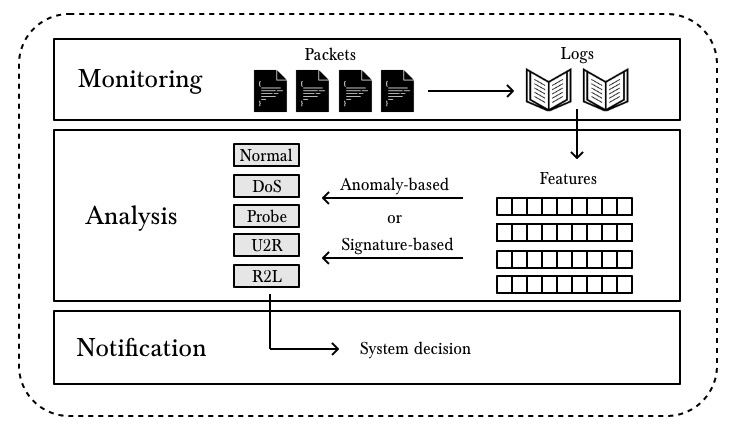
\includegraphics[width=.95\textwidth]{parts/chap-2/img-2/ids-model.jpg}
    \caption{General structure of an intrusion detection system. The different attack classes are based here on the chapter~\ref{cha:4}.} 
    \label{img:ids-model}
\end{figure}

\subsection{Extraction of features}
Packets to be analyzed are of huge size and cannot be analyzed as such by the IDS. They typically incorporate huge redundancy and other non-necessary information such as padding. The idea of feature reduction is to reduce the packets to a limited number of features, representing as much non-redundant information as possible. Examples of features extracted consist of the connection length, the protocol used, the number of bytes transferred from the source to the destination and inversely.


\subsection{Pattern analysis}
The goal of the analysis of the IDS is to categorize the packets into different classes, typically a normal class and some different attack classes. As stated in the introduction, this can be done by two different manners based on a signature (\emph{signature-based}) and using some statistical rules (\emph{anomaly-based}). In this thesis, we will interest us to anomaly-based IDS, more specifically using classification machine-learning algorithms. The goal is that some party is able to classify its data based (query) on trained machine-learning algorithms from another party. Furthermore, these algorithms have to be privacy-friendly in the sense that nor the query, nor the information resulting from the training to be revealed. This chapter aims at describing the two main machine-learning algorithms used without any consideration of the privacy-friendliness that will covered in chapter~\ref{cha:3}.

\FloatBarrier